El lenguaje de programación utilizado es Python, elegido por su sintaxis clara y fácil de leer, lo que permite centrarse más en la lógica del código y menos en los detalles sintácticos. Además, Python cuenta con una amplia variedad de bibliotecas y frameworks específicos para el aprendizaje automático y análisis de datos, tales como TensorFlow, Keras, PyTorch, Scikit-learn, Matplotlib, Seaborn y Pandas. Todas estas herramientas ofrecen funciones avanzadas que facilitan el desarrollo de proyectos en esta área, asi como BERT. El mismo es el modelo utilizado para el etiquetado de texto, y significa Bidirectional Encoder Representations from Transformers. Es un modelo de lenguaje preentrenado desarrollado por Google, tiene una arquitectura compuesta por múltiples capas de transformers, que son unidades básicas que procesan secuencias de entrada de manera bidireccional. Esto significa que el modelo puede capturar el contexto de una palabra en una oración teniendo en cuenta tanto las palabras que la preceden como las que la siguen, lo que lo hace extremadamente efectivo para una amplia gama de tareas de procesamiento del lenguaje natural. Esto se logra mediante el entrenamiento del modelo en dos tareas: 

\begin{itemize}
\item El modelado de lenguaje enmascarado (Masked Language Modeling, MLM) que ocurre durante el entrenamiento, donde BERT recibe una secuencia de palabras de entrada y algunas de estas palabras son enmascaradas aleatoriamente. La tarea del modelo es predecir qué palabra falta en cada lugar enmascarado, lo que obliga al modelo a comprender el contexto de las palabras en una oración para poder predecir la palabra enmascarada con precisión. Ver figura \ref{fig:nlp8}

\item Predicción de la siguiente oración: Además del MLM, BERT también se entrena en una tarea de predicción de la siguiente oración. Se le proporcionan dos oraciones y el modelo debe predecir si la segunda oración sigue a la primera en un contexto coherente o no.
\end{itemize}

\begin{figure}[h!]
	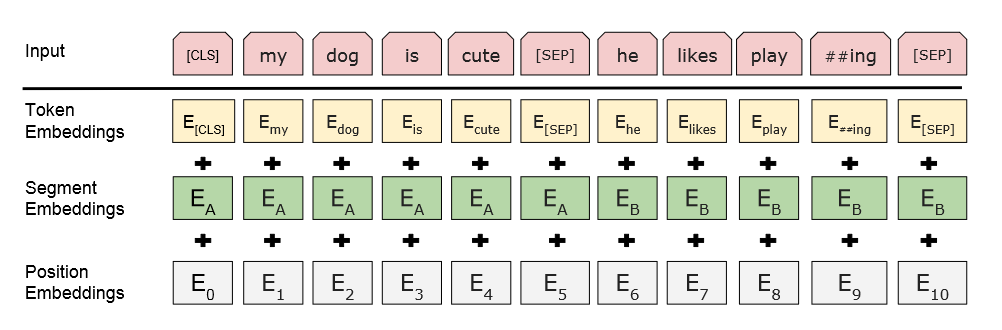
\includegraphics[width=0.65\textwidth]{capitulo3/figuras/nlp8.png}
	\caption{Representacion de entradas en BERT.
		\\\textit{Fuente: Extraído de} \protect\cite[p. 5]{devlin2018bert} }
	\label{fig:nlp8}
\end{figure}

Para este proyecto, se utilizó la versión específica de BERT denominada ``bert\_uncased\_L-4\_H-512\_A-8'', una de las 24 variantes del conjunto ``BERT miniatura''. Estos modelos son versiones más compactas del BERT original, con una arquitectura reducida en comparación con BERT base o BERT grande, como se muestra en la tabla \ref{tbl:1}. Esto significa que tienen menos parámetros y requieren menos recursos computacionales para su entrenamiento y ejecución. Dado que los recursos necesarios para trabajar con un BERT base no están disponibles para este proyecto, utilizar este modelo compacto resultó extremadamente útil.

El modelo ``bert\_uncased\_L-4\_H-512\_A-8'' se entrena con texto en minúsculas, de ahí su denominación ``uncased''. Cuenta con cuatro capas (indicadas por ``L-4''), una dimensión de representación oculta de 512 en cada capa (indicada por ``H-512'') y utiliza ocho cabezas de atención en la capa de atención multi-cabeza (representadas por ``A-8'').

\begin{table}[!ht]
	\centering
	\caption{Representacion de versiones de BERT
		\\\textit{Fuente: Elaboracion Propia}}
	\begin{tabular}{|c|>{\centering\arraybackslash}m{2.5cm}|>{\centering\arraybackslash}m{2.5cm}|>{\centering\arraybackslash}m{3cm}|>{\centering\arraybackslash}m{2.5cm}|}
		\hline
		\textbf{} & \textbf{H=128} & \textbf{H=256} & \textbf{H=512} & \textbf{H=768} \\ \hline
		\textbf{L=2} & \makecell{2/128 \\ (BERT-Tiny)} & 2/256 & 2/512 & 2/768 \\ \hline
		\textbf{L=4} & 4/128 & \makecell{4/256 \\ (BERT-Mini)} & \makecell{4/512 \\ (BERT-Small)} & 4/768 \\ \hline
		\textbf{L=6} & 6/128 & 6/256 & 6/512 & 6/768 \\ \hline
		\textbf{L=8} & 8/128 & 8/256 & \makecell{8/512\\(BERT-Medium)} & 8/768 \\ \hline
		\textbf{L=10} & 10/128 & 10/256 & 10/512 & 10/768 \\ \hline
		\textbf{L=12} & 12/128 & 12/256 & 12/512 & \makecell{12/768 \\ (BERT-Base)} \\ \hline
	\end{tabular}
	\label{tbl:1}
\end{table}


Para cada tarea que se desee realizar con BERT, es crucial seleccionar los mejores hiperparámetros de ajuste a partir de las siguiente tabla \ref{tbl:2}:

\begin{table}[!ht]
	\centering
	\begin{tabular}{|c|c|}
		\hline
		\textbf{Hiperparametros} & \textbf{Valores} \\ \hline
		Tamaños de lote & 8, 16, 32, 64, 128 \\ \hline
		Tasas de aprendizaje & 3e-4, 1e-4, 5e-5, 3e-5 \\ \hline
		Número de épocas &  1, 2, 3, 4, 5 \\ \hline
		Tipo de capa de preprocesamiento & Según el modelo a usar \\ \hline
	\end{tabular}
	\caption{Detalle de hiperparametros y sus valores en BERT
		\\\textit{Fuente: Elaboracion Propia}}
	\label{tbl:2}
\end{table}

En este proyecto, para la tarea de etiquetado de los conjuntos de datos, se optó por un modelo de preprocesamiento ya entrenado específicamente seleccionado. La configuración específica incluyó:

\begin{itemize}

\item Capa de preprocesamiento: Una capa codificadora entrenable que se actualiza durante el entrenamiento(en-uncased-preprocess-version-3).
\item Capa de abandono: Con una tasa de abandono del 10\%.
\item Capa densa: Con una función de activación softmax para la clasificación múltiple.
\item Tamaño de lote: 32, lo que significa que los datos se dividen en lotes más pequeños con ese tamaño.
\item Tasa de aprendizaje: 3e-5.
\item Optimizador: AdamW.
\item Número de épocas: 5.

\end{itemize}

Para evaluar el modelo, se obtuvieron la pérdida y la precisión del modelo en el conjunto de prueba.

El entrenamiento del modelo BERT, el proceso de etiquetado de datos y la creación y entrenamiento de modelos de redes convolucionales se llevaron a cabo utilizando Google Colab (abreviatura de Colaboratory), una plataforma en línea proporcionada por Google. Colab permite escribir y ejecutar código Python en un entorno de cuaderno basado en la nube de forma gratuita como se muestra en la figura \ref{fig:bertito}. Está diseñado para facilitar la colaboración en proyectos de ciencia de datos y aprendizaje automático, así como para el desarrollo y experimentación con código Python sin necesidad de configurar un entorno local.

Google Colab ofrece acceso gratuito a recursos de cómputo en la nube, incluidas unidades de procesamiento gráfico (GPU) y unidades de procesamiento tensorial (TPU). Estos recursos fueron utilizados para el etiquetado de los conjuntos de datos. Sin embargo, el uso gratuito de CPU, GPU y TPU tiene limitaciones. Estas limitaciones se hicieron evidentes al entrenar el modelo BERT con grandes cantidades de datos, ya que el proceso requería mucho más tiempo de entrenamiento y el entorno se desconectaba, dejando el entrenamiento incompleto. Para evitar este problema, se adquirió el paquete Colab Pro, el cual garantiza que el entorno de ejecución no se desconecte y permite que BERT complete su entrenamiento sin interrupciones.

\begin{figure}[h!]
	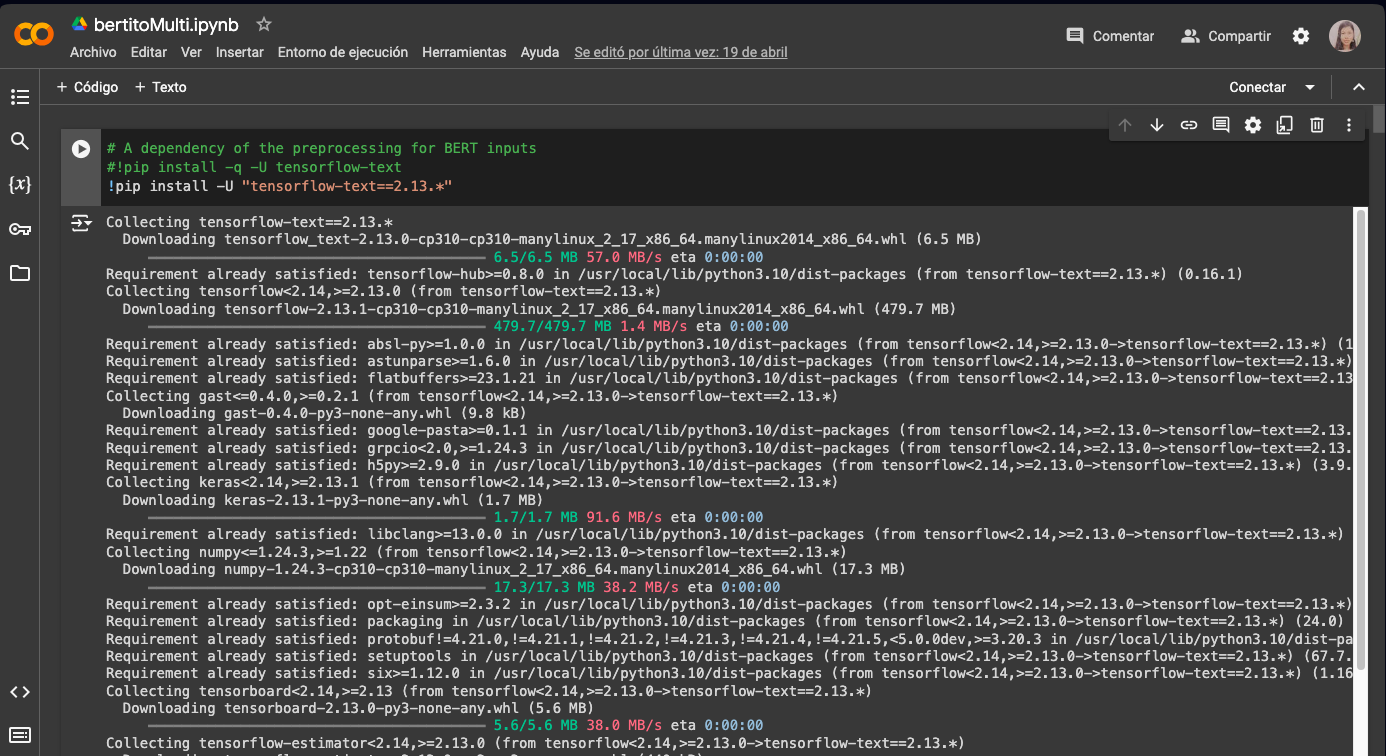
\includegraphics[width=1\textwidth]{capitulo5/figuras/bertito.png}
	\caption{Formato de cuaderno colab instalando libreria tensorflow-text-2.13
		\\\textit{Fuente: Elaboracion Propia}}
	\label{fig:bertito}
\end{figure}

Para la creación de los modelos de redes neuronales convolucionales se utilizó Keras, una API de alto nivel recomendada para TensorFlow a partir de su versión 1.14. Keras es una biblioteca de código abierto para la creación y entrenamiento de modelos de redes neuronales en Python. Es conocida por su facilidad de uso, ya que proporciona una interfaz de alto nivel que simplifica la construcción y el entrenamiento de modelos de redes neuronales. Los modelos de Keras se construyen utilizando capas que se pueden apilar o combinar de diversas formas para crear arquitecturas complejas.

A continuación, se detallan las versiones y bibliotecas utilizadas:

\begin{itemize}

\item Keras: 2.15.0
\item Matplotlib: 3.1.1
\item NumPy: 1.17.4
\item Python: 3.11.4
\item TensorFlow: 2.13.0 (para el modelo BERT)
\item Tensor-text: 2.13.0 (para el modelo BERT)
\item TensorFlow: 2.15.0 (para otros modelos)

\end{itemize}